\documentclass[tikz]{standalone}
\begin{document}
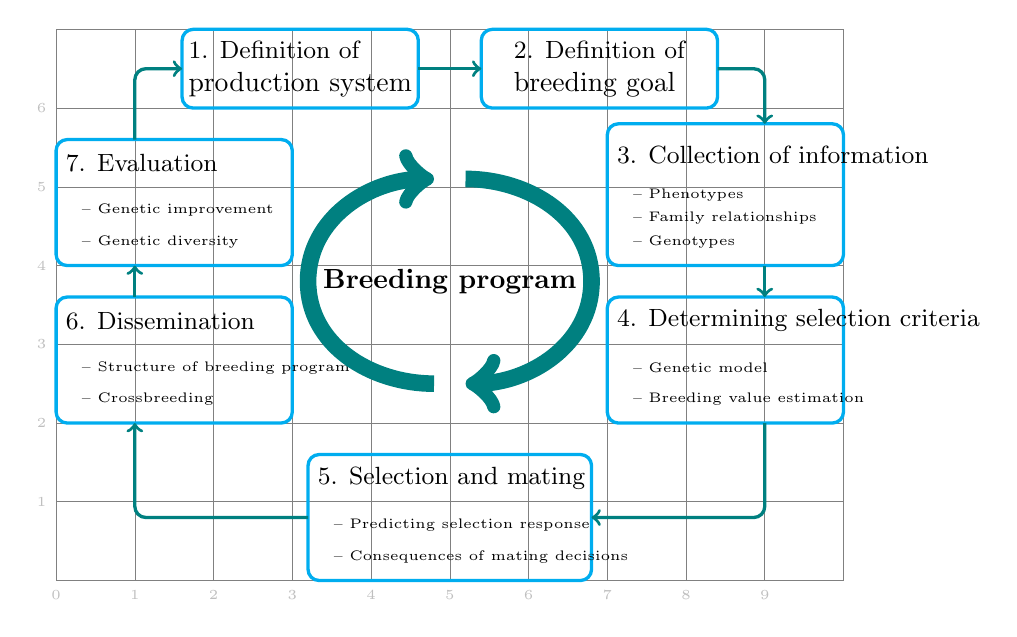
\begin{tikzpicture}
  \draw[help lines] (0,0) grid (10,7);
  \foreach \x in {0, 1, ..., 9} \node[below, gray!50] at (\x,0){\tiny{\x}};
  \foreach \y in {1, 2, ..., 6} \node[left, gray!50] at (0,\y){\tiny{\y}};
  \draw[cyan, very thick, rounded corners] (3.2, 0) rectangle (6.8,1.6);
  %\node[text width=4cm, right] at (2.7, 0.8){\small 
  %  \begin{enumerate}
  %    \setcounter{enumi}{4}
  %  \item Selection and mating
  %    \begin{itemize}
  %    \item Prediction selection response
  %    \item Consequences of mating decisions
  %    \end{itemize}
  %  \end{enumerate}
  %  };
  \node[right] at (3.2, 1.3) {\small 5. Selection and mating};
  \node[right] at (3.4, 0.7){\tiny -- Predicting selection response};
  \node[right] at (3.4, 0.3){\tiny -- Consequences of mating decisions};
  \draw[cyan, very thick, rounded corners] (0, 2) rectangle (3, 3.6);
  \node[right] at (0, 3.3) {\small 6. Dissemination};
  \node[right] at (0.2, 2.7) {\tiny -- Structure of breeding program};
  \node[right] at (0.2, 2.3) {\tiny -- Crossbreeding};
  \draw[cyan, very thick, rounded corners] (0, 4) rectangle (3, 5.6);
  \node[right] at (0, 5.3) {\small 7. Evaluation};
  \node[right] at (0.2, 4.7) {\tiny -- Genetic improvement};
  \node[right] at (0.2, 4.3) {\tiny -- Genetic diversity};
  \draw[cyan, very thick, rounded corners] (1.6, 6) rectangle (4.6,7);
  \node[align=left] at (3.1,6.5) {\small 1. Definition of\\production system};
  \draw[cyan, very thick, rounded corners] (5.4, 6) rectangle (8.4,7);
  \node[align=left] at (6.9, 6.5) {\small 2. Definition of \\breeding goal};
  \draw[cyan, very thick, rounded corners] (7, 4) rectangle (10, 5.8);
  \node[right] at (7, 5.4) {\small 3. Collection of information};
  \node[right] at (7.2, 4.9) {\tiny -- Phenotypes};
  \node[right] at (7.2, 4.6) {\tiny -- Family relationships};
  \node[right] at (7.2, 4.3) {\tiny -- Genotypes};
  \draw[cyan, very thick, rounded corners] (7, 2) rectangle (10, 3.6);
  \node[right] at (7, 3.3) {\small 4. Determining selection criteria};
  \node[right] at (7.2, 2.7) {\tiny -- Genetic model};
  \node[right] at (7.2, 2.3) {\tiny -- Breeding value estimation};
  \node at (5, 3.8) {\textbf{Breeding program}};
  \draw[teal, line width=6, ->](4.8, 2.5) to [out=180, in=-90] (3.2, 3.8) to [out=90, in=180] (4.8, 5.1);
  \draw[teal, line width=6, ->](5.2, 5.1) to [out=0, in=90] (6.8, 3.8) to [out=-90, in=0] (5.2, 2.5);
  \draw[teal, very thick, ->, rounded corners] (3.2, 0.8)--(1, 0.8)--(1,2);
  \draw[teal, very thick, ->, rounded corners] (1, 3.6)--(1,4);
  \draw[teal, very thick, ->, rounded corners] (1, 5.6)--(1, 6.5)--(1.6, 6.5);
  \draw[teal, very thick, ->, rounded corners] (4.6, 6.5)--(5.4,6.5);
  \draw[teal, very thick, ->, rounded corners] (8.4, 6.5)--(9,6.5)--(9,5.8);
  \draw[teal, very thick, ->, rounded corners] (9,4)--(9,3.6);
  \draw[teal, very thick, ->, rounded corners] (9,2)--(9,0.8)--(6.8,0.8);
\end{tikzpicture}
\end{document}
